\section{Induced Relational Views}
\label{sec:Induced Relational Views}
In this section, we discuss the idea of induced relational views, central to our induced relational GCN framework developed in~\Cref{sec:gcn}.
First, in~\Cref{sub:Induced Views}, we introduce potential strategies for selecting the accepted answer given a question. We show how each strategy induces a graph $G$ on the question-answer $(q,a)$ tuples. Next, in~\Cref{sub:Generalized Views}, we show how each of these example strategies is an instance of an equivalence relation; our framework generalizes to incorporate any such relation.

\begin{figure}[h]
    \centering
    \begin{subfigure}{0.25\textwidth}
        \centering
        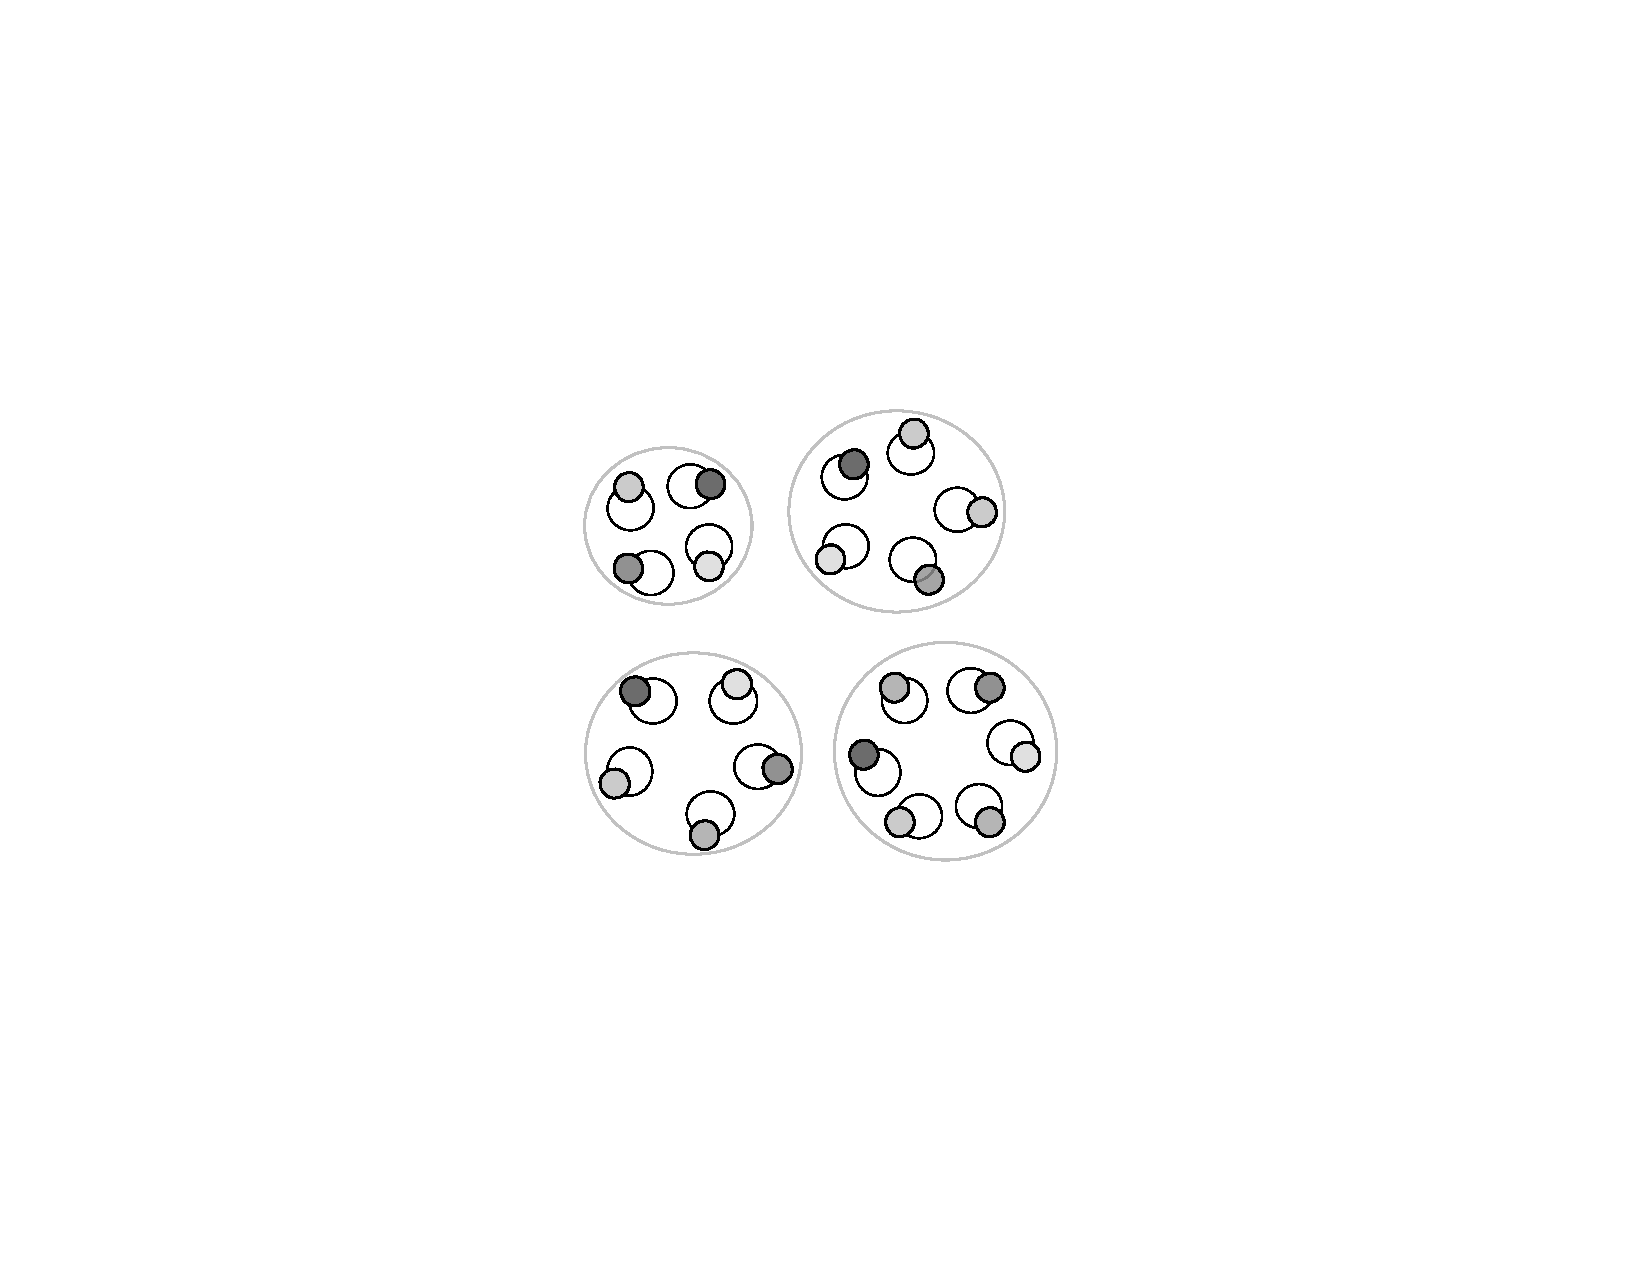
\includegraphics[scale=0.4]{figures/reflex_updated}
            \caption{Reflexive}
            \label{fig:reflexive}
    \end{subfigure}%
    \begin{subfigure}{0.27\textwidth}
        \centering
        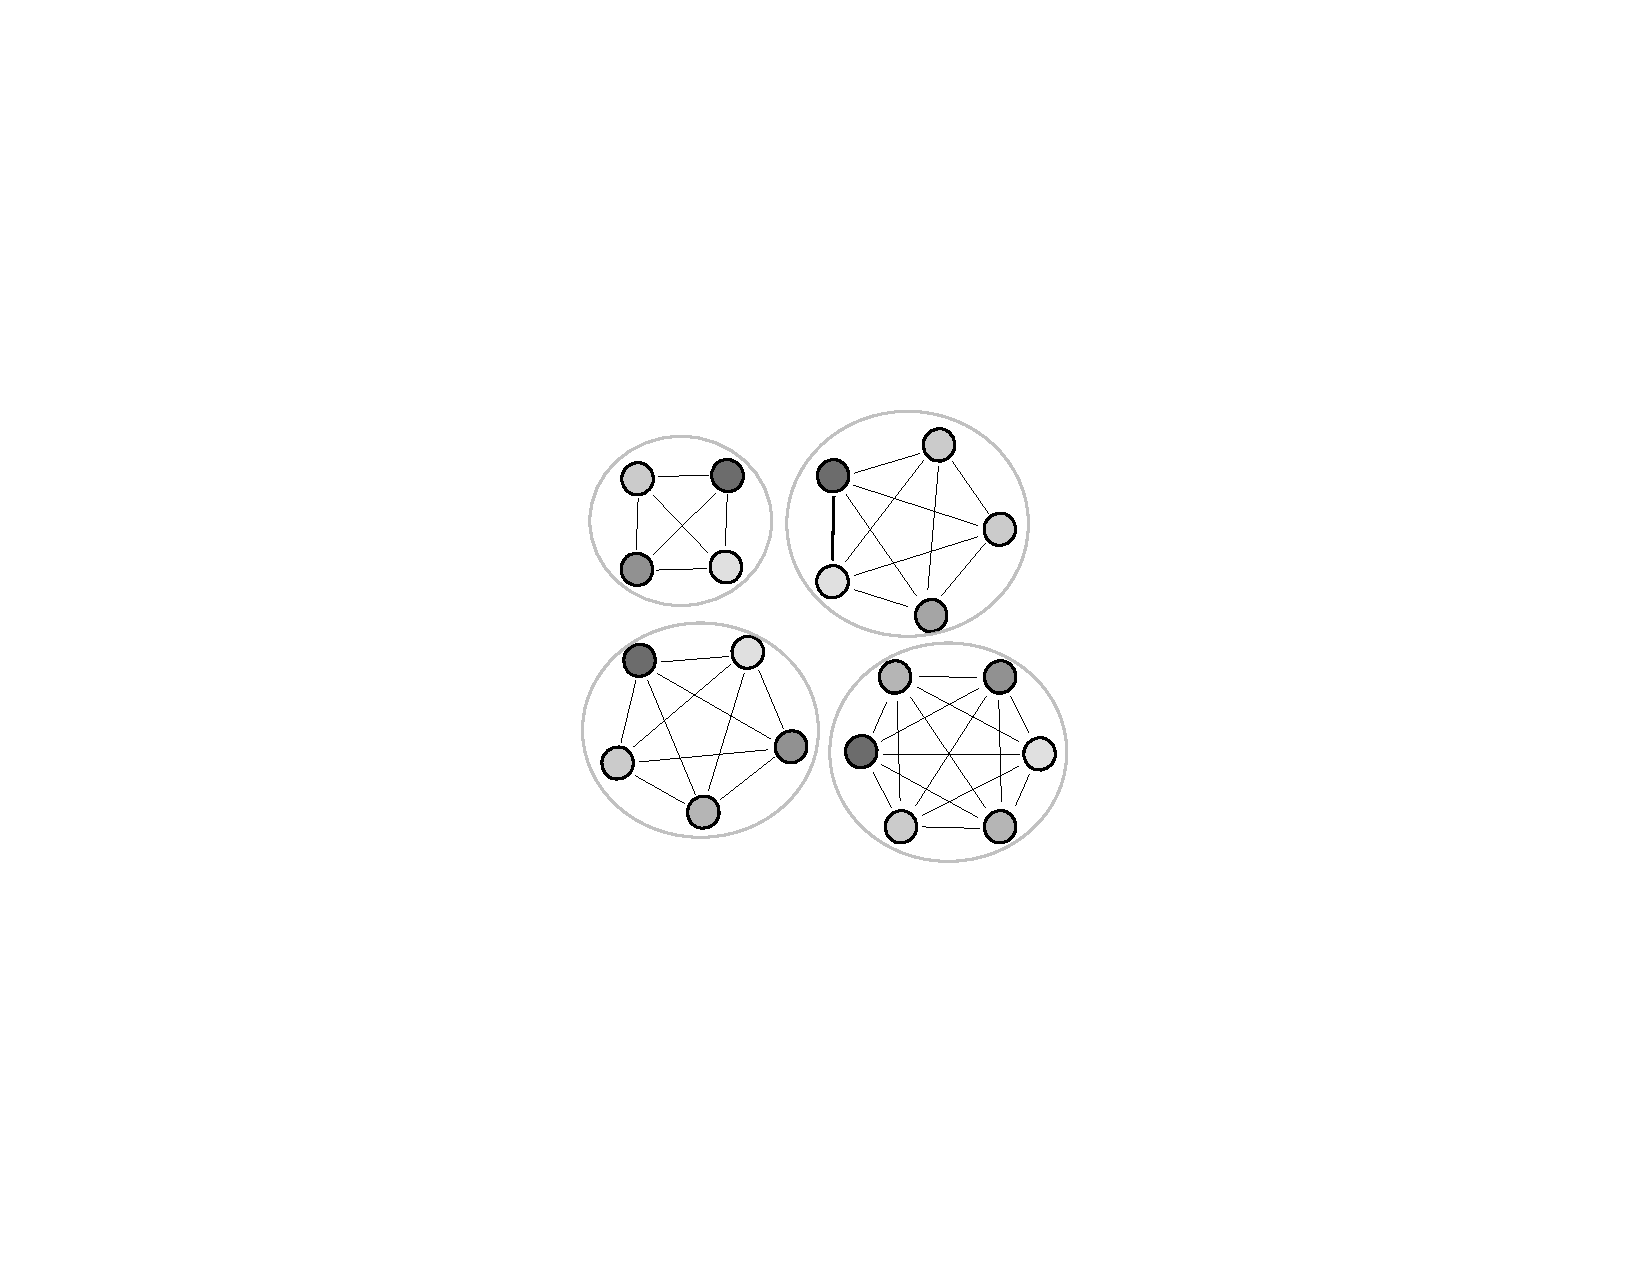
\includegraphics[scale=0.4]{figures/Contrast_circle}
        \caption{Contrastive}
        \label{fig:contrastive}
    \end{subfigure}%
    \begin{subfigure}{0.25\textwidth}
        \centering
        %\includegraphics[width=\linewidth,height=5cm]{figures/drawing}
            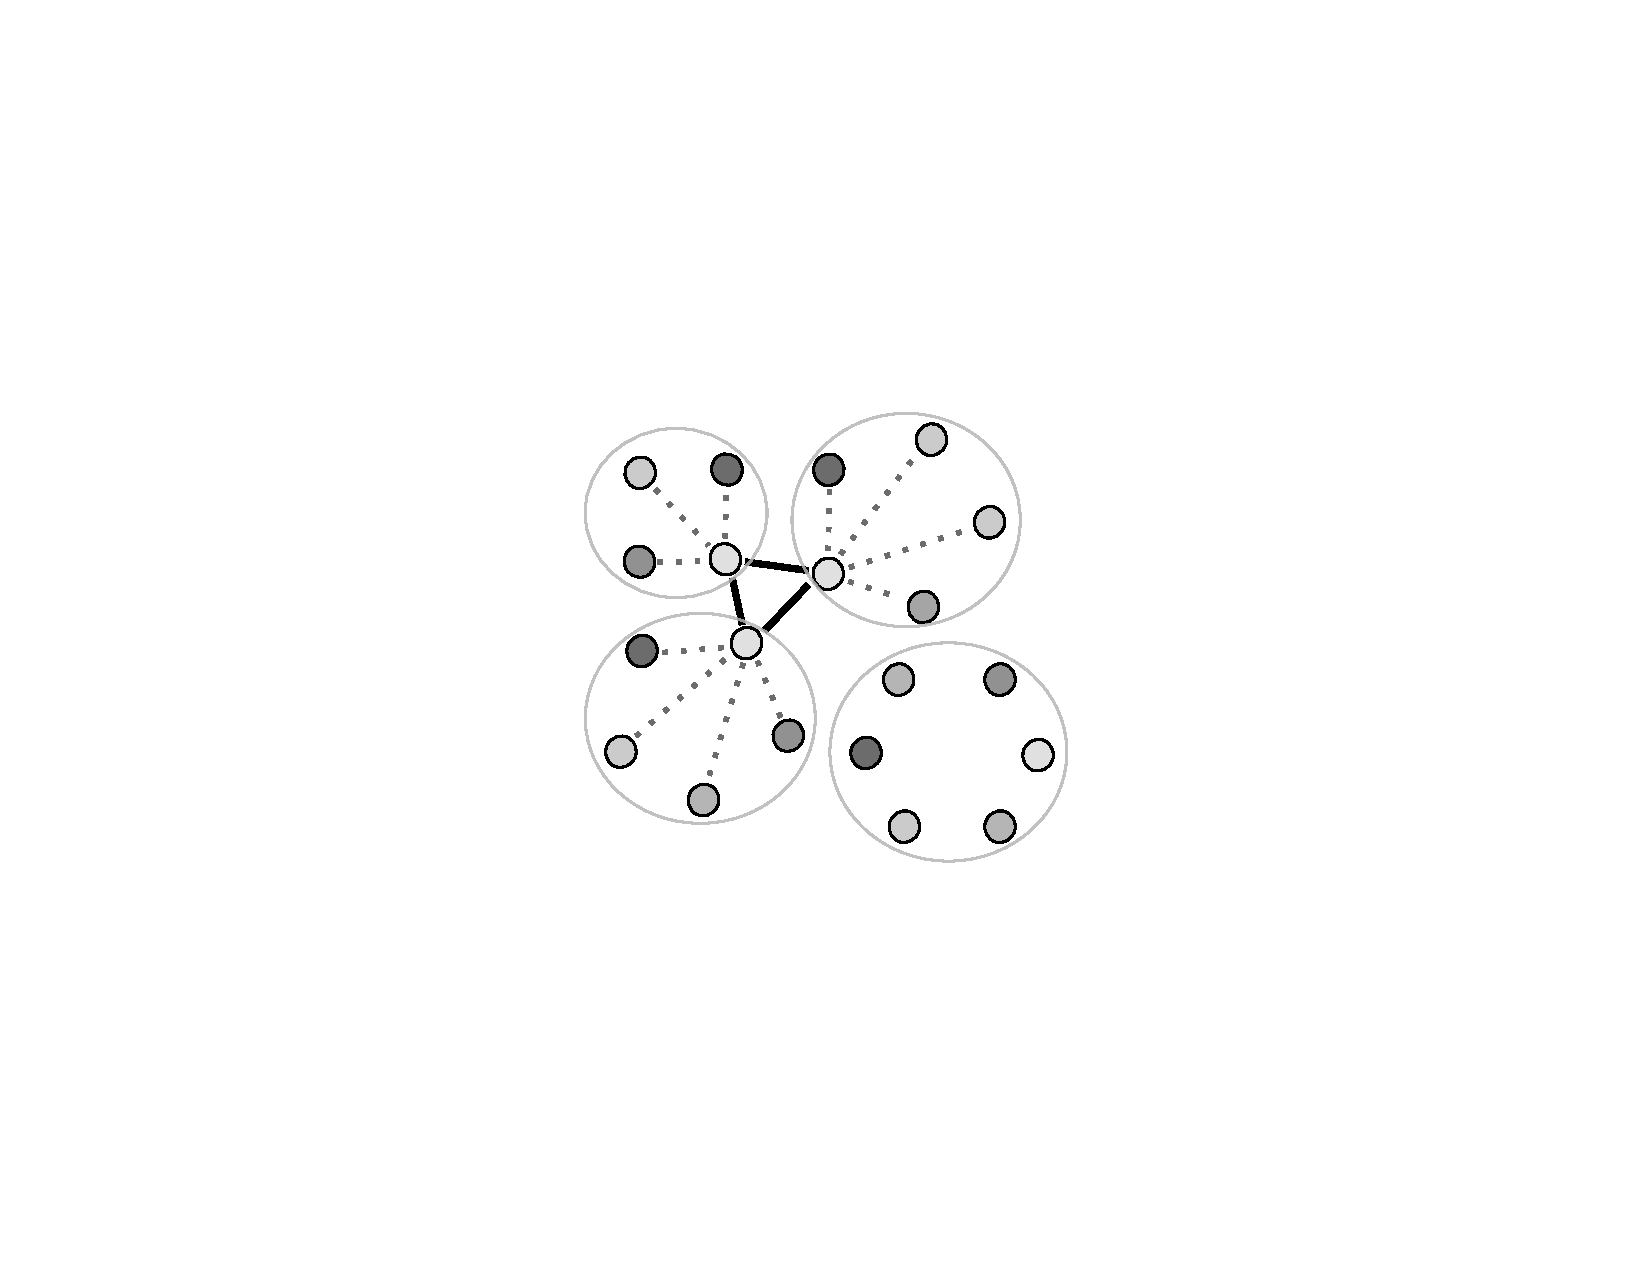
\includegraphics[scale=0.4]{figures/similarContrast_old}
      \caption{Similar Contrast}
      \label{fig:similar}
        \end{subfigure}%
    \caption{\label{fig:relation} Reflexive(~\cref{fig:reflexive}), Contrastive (~\cref{fig:contrastive}) and Similar Contrast (~\cref{fig:similar}) relations among $(q,a)$ tuples. Reflexive assumes no dependence on other answers for prediction. Contrastive compares between all answers to a question;  Similar Contrast connects answers across questions if they contrasts with other answers similarly. Solid lines show the similarity relation while dotted lines signify the contrast. The contrast is only significant in three questions.}
\end{figure}

\subsection{Constructing Induced Views}
\label{sub:Induced Views}


In this section, we discuss in detail four example strategies that can be used by the individual posting the question to label an answer as `accepted.'
Each of the $S_i \in \mathbf{S}$ strategies \textit{induces} a graph $G_i = (V, E_i)$ (also referred to as a relational view).
In each graph $G_i$, a vertex $v \in V$ corresponds to a tuple $(q,a)$ and an edge $e \in E_i, E_i \subseteq V \times V$ connects two tuples that are matched under that strategy.
Note that each $G_i$ has the same vertex set $V$, and the edge sets $E_i$ are strategy dependent. Each strategy employs one of the three different relation types---reflexive, contrastive, and similar---to connect the tuples. We use one reflexive strategy, one contrastive, and two similar strategies.
~\Cref{fig:relation} summarizes the three relations. Below, we organize the discussion by relation type.

\textbf{Reflexive:}
\label{sub:Reflexive}
A natural strategy is to examine each $(q,a)$ tuple in isolation and then assign a label $y_{q,a} \in \{-1,+1 \}$ corresponding to `not accepted' or `accepted.' In this case, $y_{q,a}$ depends on only the features of $(q,a)$. This is a \emph{Reflexive} relation, and the corresponding graph $G_r = (V,E_r)$ has a specific structure. In particular, in this graph $G_r$, we have only self-loops, and all edges $e \in E_r$ are of the type $(v,v)$. That is, for each vertex $v \in V$, there are no edges $(v,u)$ to any other vertices $u\neq v \in V$. Much of the prior work on feature driven answer selection~\cite{BurelMA16,  JendersKN16, TianZL13, TianL16} adopts this view.

\textbf{Contrastive:}
\label{sub:Contrastive}
A second strategy is to examine answers \textit{in relation} to other answers to the same question and label one such answer as `accepted.' Thus the second strategy \textit{contrasts} $(q,a)$, with other tuples in  $(q,a'), q \in \mathcal{Q}; a, a' \in \mathcal{A}_q; a'\neq a$. This is a \emph{Contrastive} relation and the corresponding graph $G_c = (V,E_c)$ has a specific structure. Specifically, we define an edge $e \in E_c$ for all $(q,a)$ tuples for the same question $q \in \mathcal{Q}$. That is, if  $v = (q_1, a_1), u=(q_2, a_2)$, $e=(u, v) \in E_c \iff q_1=q_2$. Intuitively, the contrastive relation induces cliques connecting all answers to the same question. Introducing contrasts between vertices sharpens differences between features, an effect (described in more detail in~\Cref{subsec:contrast}) we term \emph{Discriminative Feature Magnification}. Notice that the contrastive relation is distinct from graphs with signed edges (e.g.,~\cite{signedgcn}). In our framework, the contrast is a \textit{neighborhood} property of a vertex, whereas in~\cite{signedgcn}, the negative sign is a property of an \textit{edge}.

\textbf{Similar Contrasts:}
\label{sub:Similar}
A third strategy is to identify \textit{similar} $(q,a)$ tuples \textit{across} questions. Prior work~\cite{Wu2016} indicates that individuals on StackExchange use diverse strategies to contribute answers. Experts (with a high reputation) tend to answer harder questions, while new members (with low reputation)  looking to acquire reputation tend to be the first to answer a question.

How might similarity by contrast work? Consider two individuals Alice and Bob with \textit{similar} reputations (either high or low) on StackExchange, who contribute answers $a_A$ and $a_B$ to questions $q_1$ and $q_2$ respectively. If Alice and Bob have high reputation difference with other individuals who answer questions $q_1$ and $q_2$ respectively, then it is likely that $(q_1, a_A)$ and $(q_2, a_B)$ will share the same label (if they are both experts, their answers might be accepted, if they are both novices, then this is less likely). However, if Alice has a high reputation difference with other peers who answer $q_1$, \textit{but Bob does not have that difference} with peers who answer $q_2$, then it is less likely that the tuples $(q_1, a_A)$ and $(q_2, a_B)$ will share the label, even though the reputations of Alice and Bob are similar.

Thus, the key idea of the \emph{Similar Contrasts} relation is that link tuples that are  \textit{similar in how they differ} with other tuples. We construct the graph $G_s = (V, E_s)$ in the following manner. An edge $e = (v,u)$ between tuples $v$ and $u$ exists if the similarity $s(v,u)$ between tuples $v,u$ exceeds a threshold $\delta$. We define the similarity function $s(\cdot , \cdot)$ to encode similarity by contrast. That is, $e=(v,u) \in E_s \iff s(v,u) \geq \delta$.

\begin{figure}[htb]
  \centering
  \begin{subfigure}{0.4\textwidth}
    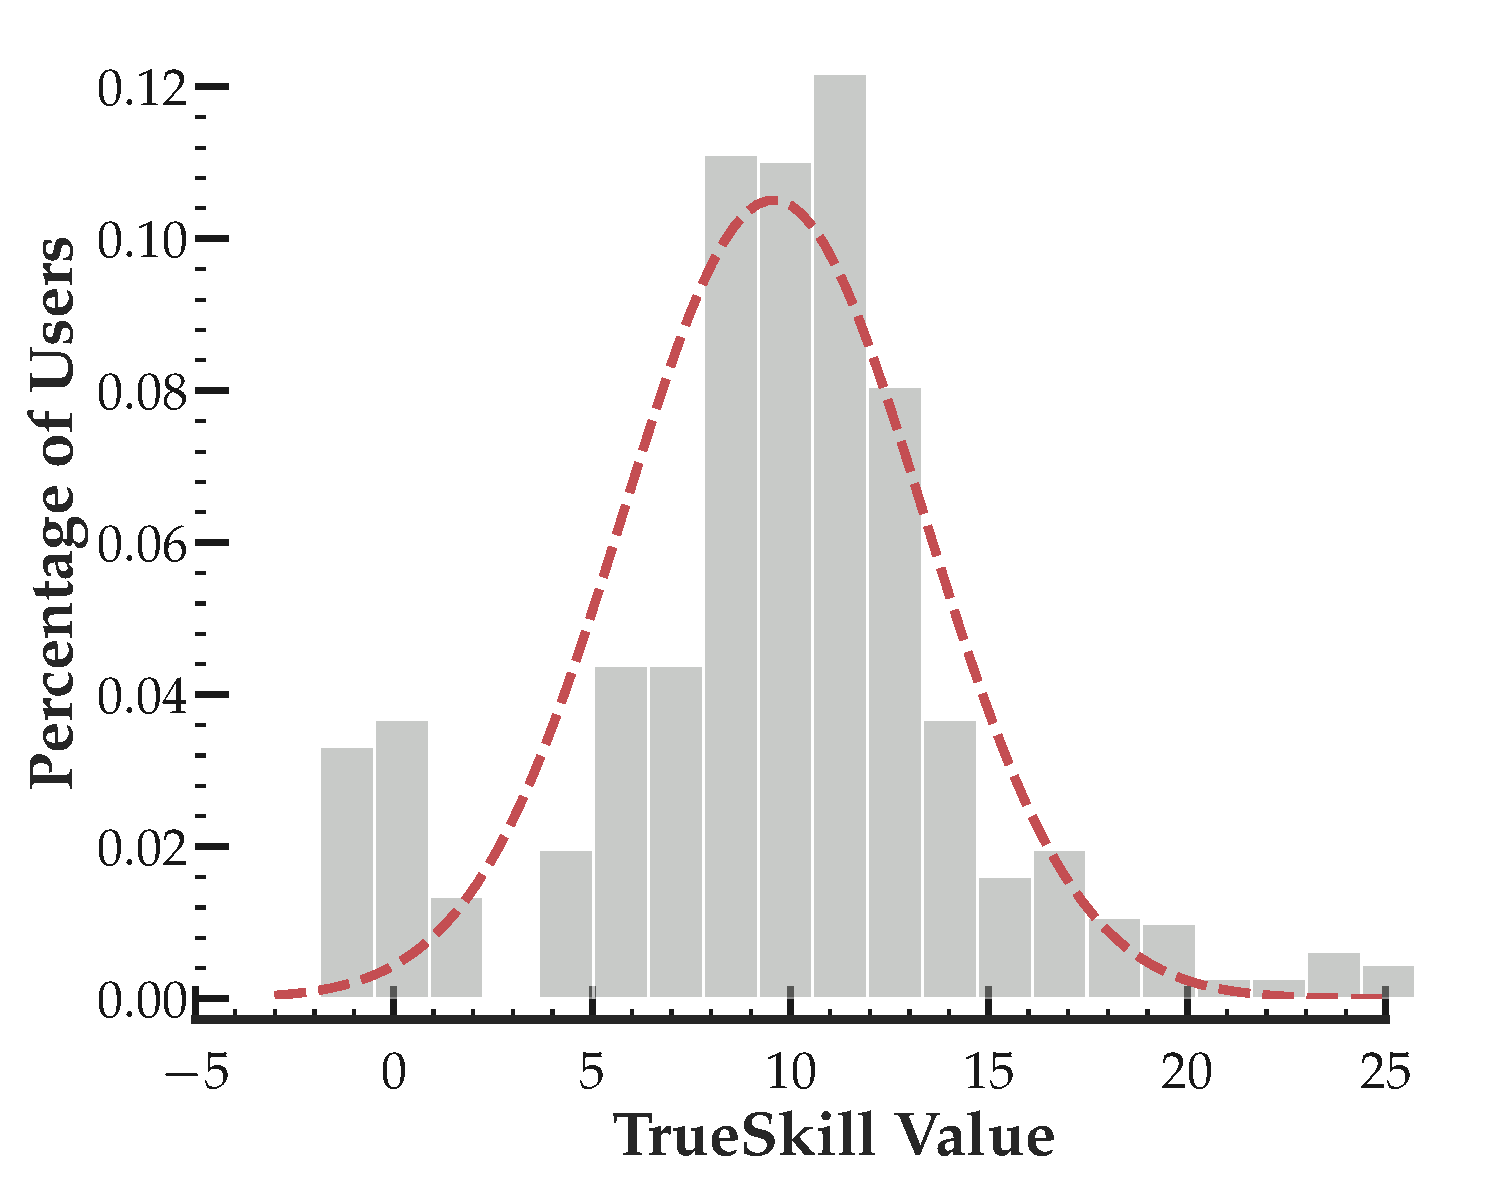
\includegraphics[height=5cm,width=\textwidth]{figures/TrueSkill}
    \caption{TrueSkill Distribution}\label{fig:trueskill}
  \end{subfigure}%
  \begin{subfigure}{0.4\textwidth}
    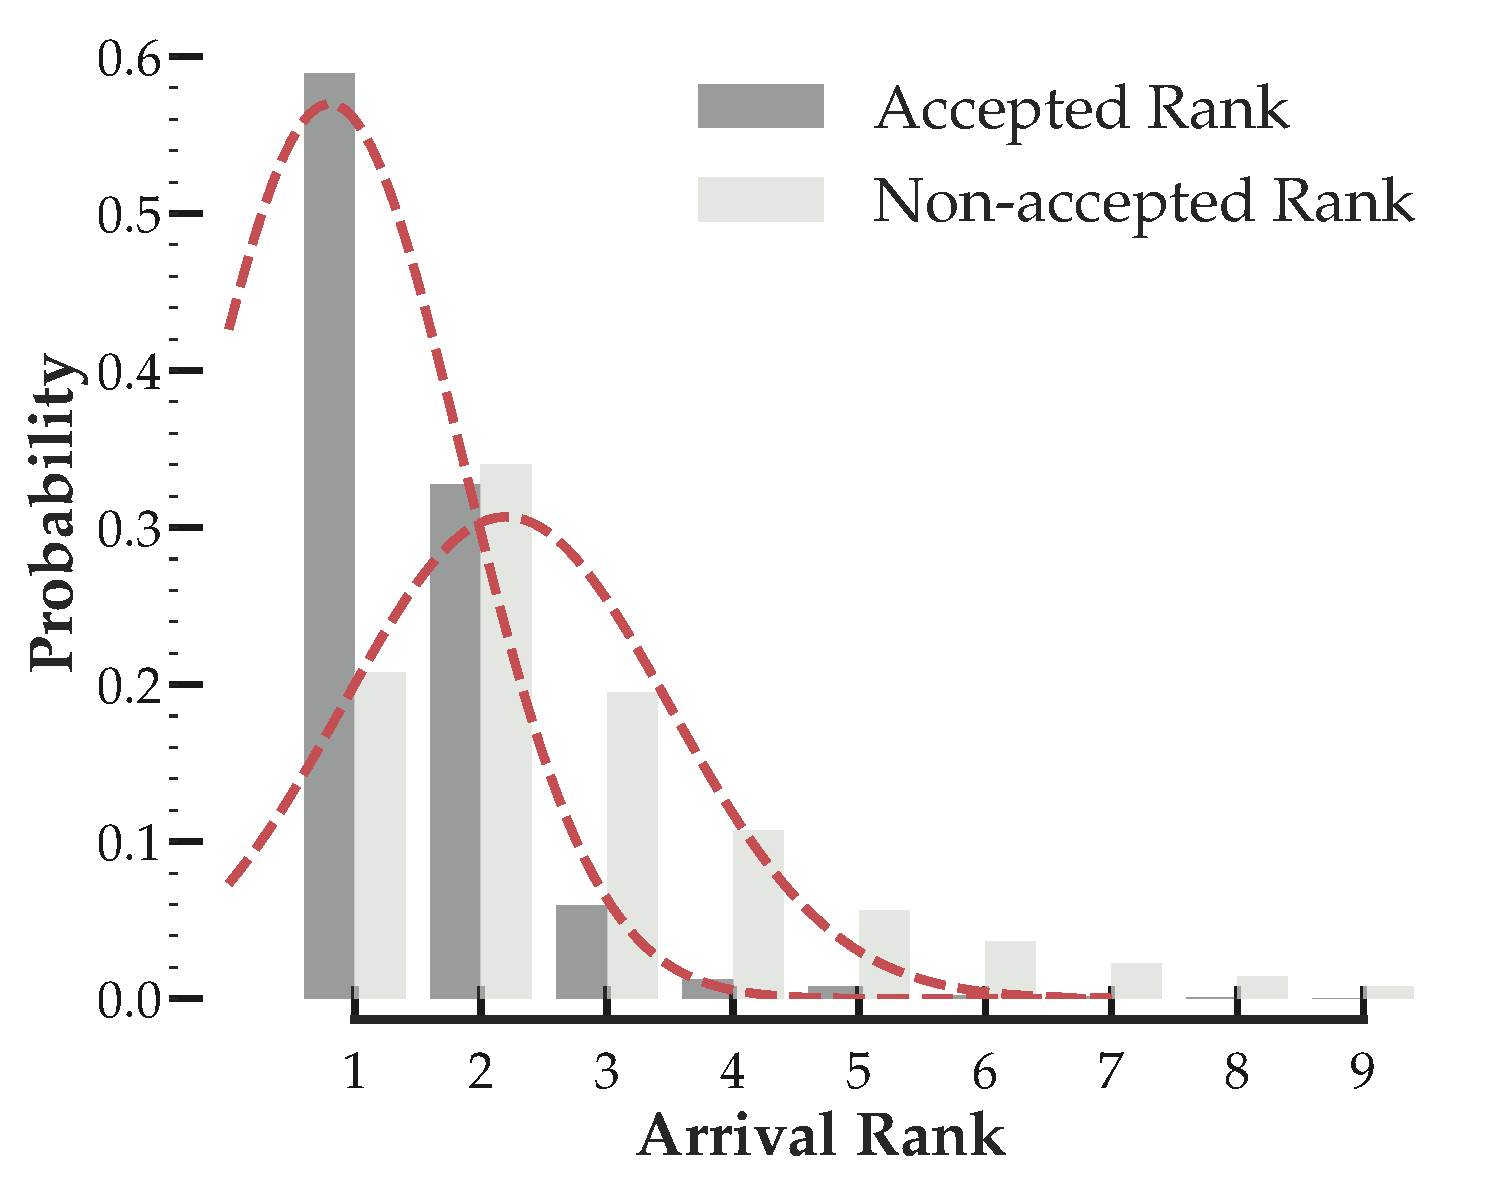
\includegraphics[height=5cm,width=\textwidth]{figures/ArrivalRank}
    \caption{ArrivalRank Distribution}\label{fig:arrival}
  \end{subfigure}
  \caption{\label{fig:similarcontrastsempirical} Distribution of the TrueSkill values of users and ArrivalRank of accepted answers and non-accepted answers for the movie StackExchange. Early answers are more likely to be accepted and variance of TrueSkill similarity across users is high.}
\end{figure}


Motivated by~\cite{Wu2016} and our empirical analysis (\cref{fig:similarcontrastsempirical}), we consider two different views that correspond to the similar contrast relation. The \emph{TrueSkill Similarity} view connects all answers authored by a user where her skill (computed via Bayesian TrueSkill~\cite{TrueSkill06})) differs from competitors by margin $\delta$. We capture both cases when the user is less or more skilled than her competitors. Under this view, we connect answers authored by a specific user, where the difference in his skill over peers is greater than margin $\delta$. Specifically, if the user authors answers $a, a'$ to questions $q, q'$, we create a link between $a$ and $a'$ if
\begin{align}
 \lvert S_{u,a} - S_{u, b} \rvert &> \delta; \forall b \in \mathcal{A}_(q) \\
 \lvert S_{u,a'} - S_{u, c} \rvert &> \delta; \forall c \in \mathcal{A}_(q')
\end{align}
where $S_{u,a}$ is the skill value for the user who authored answer $a$. Similarly, a link is created for the opposite case when difference is less than $-\delta$.
We estimate the user skill values with the TrueSkill rating system (\url{https://pypi.org/project/trueskill/}) computed from their historic performance in the community. TrueSkill values are normally distributed among users (\cref{fig:trueskill}).

In the \emph{Arrival Similarity} view, we connect answers across questions based on the similarity in the relative time of their arrival (posting timestamp).
The temporal arrival patterns of answers are correlated to their acceptance probabilities (\cref{fig:arrival}). For a specific user authoring answers $a, a'$ to questions $q, q'$, we establish a link between these answers if
\begin{align}
 \lvert T_{a} - T_{b} \rvert &> \gamma \times \max(T_{b}); \forall b \in \mathcal{A}_(q) \\
 \lvert T_{a'} - T_{c} \rvert &> \gamma \times \max(T_{c}); \forall c \in \mathcal{A}_(q')
\end{align}
where $T_{a}$ represents the relative time-gap between answer $a$ and the question $q$. Conversely, we create links when difference is less than $-\gamma \times \max(T_{b})$.

We hypothesize that a similar answering schedule indicates similar user confidence or skill across questions.
Notice that two Similar Contrast views have different edge ($E$) sets since the corresponding similarity functions are different. Notice also, that the two similarity function definitions are transitive.
 \footnote{One trivial way of establishing similarity is co-authorship i.e., connect all $(q,a)$ tuples of a user (probably on the same topic) across different questions.
Note that the accepted answer is labeled relative to the other answers. As the competing answers are different in each question, we can not trivially assume acceptance label similarity for all coauthored answers. In our experiments, co-authorship introduced a lot of noisy links in the graph leading to worse performance.}

\subsection{Generalized Views}
\label{sub:Generalized Views}
Now we present the general case of the induced view. First, notice that each of the three relation types that we consider---reflexive, contrastive, and similar---result in a graph $G_i = (V, E_i)$ comprising a set of cliques. The resulting set of cliques is not surprising, since all three relations presented here, are equivalence relations. Second, observe the semantics of how we select the tuple with the accepted answer. Within the three relations, we used two semantically different ways to assign the `accepted' answer label to a tuple. One way is to share the labels amongst all the vertices in the \textit{same clique} (used in the reflexive and the similar relations). The second is to \textit{assign label based on contrasts with other vertices} in the same clique. We can now state the organizing principle of our approach as follows.
\begin{quote}
  A generalized \textit{modular} framework: pick a meaningful equivalence relation on the $(q,a)$ tuples to induce graph comprising cliques and then apply specific label semantics within each clique.
\end{quote}

Equivalence relation results in a graph with a set of disconnected cliques. Then, within a clique, one could use application-specific semantics, different from two discussed in this paper, to label tuples as `accepted.'
Cliques have some advantages: they have well-defined graph spectra~\cite[p. 6]{Chung1997}; cliques allows for \textit{exact} graph convolution; parallelize the training as the convolution of a clique is independent of other cliques.

Thus, each strategy induces a graph $G_i=(V,E_i)$ using one of the three equivalence relations---reflexive, contrastive, and similar---and then applies one of the two semantics (`share the same label'; `determine label based on contrast').
